%%%%%%%%%%%%%%%%%%%%%%%%%%%%%
%%% PACKAGES AND SETTINGS %%%
%%%%%%%%%%%%%%%%%%%%%%%%%%%%%
\documentclass[a4paper,12pt]{article}
\usepackage{graphicx}
\usepackage{pdfpages}
\usepackage[font=small]{caption}
\usepackage{commath}
\usepackage{amsmath}
\usepackage{multirow}
\usepackage{subcaption}
\usepackage{verbatim}
\usepackage{amssymb}
\usepackage{comment}
\usepackage{parskip}
\usepackage{setspace}
\usepackage[utf8x]{inputenc} %Use Umlauts and accents
\PassOptionsToPackage{hyphens}{url}\usepackage{hyperref}

\renewcommand{\familydefault}{\sfdefault} %Use sans-serif font
\usepackage{helvet}

\linespread{1.45} %equivalent to 1.5 in word
%\onehalfspacing

\numberwithin{equation}{section}
\numberwithin{figure}{section}
\numberwithin{table}{section}

\graphicspath{{Images/}} %Places all images in folder
\usepackage[a4paper,top=2cm,bottom=2cm,left=2cm,right=2cm,marginparwidth=1cm]{geometry}
\renewcommand*\contentsname{Table of Contents}
\usepackage[nottoc]{tocbibind}


\begin{document}

\begin{figure} [t]
    \includegraphics[scale = 0.1]{Imperial}
\end{figure}



\title{\large \underline{ME3 Literature Research Project} \\ \huge Thin Films and Soap Bubbles: Death and Stability Characteristics}

\date{2nd December, 2020}
\author{Pierre Tharreau \\ CID: 01506504}
\maketitle

\begin{figure} [h]
    \centering
    \captionsetup{width=.9\linewidth}
    \includegraphics[scale = 0.55]{Cover.jpg}
    \caption*{\textit{Experimentally observed pattern formations on a soap bubble film close to rupture \cite{Shen2020}}}
\end{figure}

%\vspace*{2cm}
%\noindent
%{\bf Word count:}
%$\approx$ 69 words.

\pagenumbering{gobble}
\newpage
\pagenumbering{roman}

\section*{Abstract}
%This is the best report that has ever been written on this planet
In this LRP, we have addressed fluid thin films in the form of bubbles while referencing studies made on foams and flat films. Firstly, their stable effects were analysed such as the role of surfactants as amphiphillic molecules which adsorb to fluid interfaces. Their specific role in altering surface tension, interfacial rheology as well as the Marangoni effect was described. Following this, a timeline descibing the phenomena and events which occur during a surface bubble's lifetime was established. This includes capillary and marginal regeneration drainage mechanisms, metastable black films, rupture nucleation, hole development and aerosol production. Finally, the factors affecting bubble stability were gleaned from the phenomena described. Surfactant solubility and concentration were found to be the most influential, with fluid viscosity, amphiphile diffusivity and ambient humidity also playing a role in bubble stability. Overall, fluid thin films have been extensively studied experimentally, and models describing drainage and surface flows are in accordance with this. However, mechanisms for the onset of rupture are still disputed, and models often rely on experimentally derived statistical parameters. Further research in this area, and in role of evaporation are required.


\setcounter{page}{2}
\newpage
\section*{Project Objectives}

\begin{itemize}
    \item Define characteristics and fundamental interactions in thin films
    \begin{itemize}
        \item Role of surface tension
		\item Role and importance of surfactants
		\item Classification (bubble, anti-bubble, thin vs. thick film)
		\item Use and applications
    \end{itemize}
    \item Discuss the interactions with the external environment
    \begin{itemize}
        \item Stable bubbles (liquid structures, e.g. Marangoni effect, effect of EM fields)
		\item Bursting of bubbles (ligaments formation, holes)
    \end{itemize}
     \item Discuss how stability characteristics could be improved/changed
\end{itemize}

\newpage
\tableofcontents

%\newpage
%\section*{Nomenclature and Abbreviations}
%\addcontentsline{toc}{subsection}{Nomenclature and Abbreviations}

\newpage
\clearpage\pagenumbering{arabic}
\section{Introduction}

A multitude of questions come to mind when observing the life of a soap bubble; how does it manage to maintain stability despite appearing so fragile? what effects explain its ephemeral nature? and what happens during rupture and after the bubble has burst? This report will attempt to summarize the mechanisms and structures which soap bubbles exhibit in their life time, while gauging their effect on the stability of these curious thin films.

Strictly, a thin film is a material layer bounded on either side a fluid or solid. Although thin films involving solids are well studied and play a significant role in a wide range of industries such as electronics and bio-systems \cite{SolidThinFilms}, this report will focus on the properties and dynamics of their fluid-only counterparts. This will mainly include surface bubbles (or circular films, as cited in older works \cite{Vrij1968, VrijDiscussion1966}), but as many of their effects are shared and easier to observe with flat films and foams \cite{Braun2002}, those will also often be referenced. Indeed, foams are essentially composed of a multitude of small bubbles, each sharing film surfaces, and meeting at "Plateau" borders where fluid tends to accumulate \cite{Almgren1976}. Surface bubbles are curved thin films which sit on the bulk liquid they were created from. %mostly look at surface bubbles, as they exhibit many interesting behaviours, and they have a lot of applications (\cite{Lhuissier2010}

Firstly, we will establish the different notions and key behaviours pertinent for stable films such as surface tension and the Marangoni effect, and their intrinsic link with surfactant molecules. These tend to adsorb to fluid boundaries \cite{Gast1997} and form stabilising layer structures \cite{Mysels1968Nomenclature}. Building from this, we will essentially construct a timeline including different phenomena the bubble will experience during its lifetime: Starting with the drainage mechanisms caused by capillary and hydrostatic pressures \cite{Lhuissier2011}, causing slow Poiseuille flow when the bubble's surfaces are considered "immobile" \cite{Nierstrasz1999, Bruinsma1995, Modini2013}, to the much more common and complex Marangoni-induced marginal regeneration flows which further act to thin the film \cite{Mysels1959Book, Bhamla2017, Bruinsma1995}.

Pausing to look at a curious metastable equilibrium state, the "Newton" or "common" black film \cite{Seung2006}, which allows the film to exist at an extremely thin level, down to two surfactant atoms thick \cite{Casteletto2003}. The nucleation and position of the hole that eventually forms on the surface will then be studied \cite{ChampougnyNotBare2016, Debregeas1998}, before its opening dynamics \cite{Culick1960}, rim destabilisation (causing interesting structures like ligaments, or cracks and folds to appear \cite{Bico2015, Lhuissier2009}), and atomisation into a mist of thin aerosol particles \cite{Modini2013} are finally discussed.

\newpage
\section{Stable curved films}
\subsection{Surface tension}
Surface tension is a measurement for how strongly molecules of the same substance are attracted to each other at a fluid boundary, via intermolecular forces. It appears as a parameter or non-dimensional number in virtually every experiment, model and energetic analysis which attempts to describe the dynamics and behaviours of thin films \cite{Ida1998}. Film and bubble persistence \cite{Modini2013}, critical thickness \cite{Manev1974, Lhuissier2011} and hole rim velocity \cite{Culick1960} are just a few characteristics which utilise it. It is the driving potential behind the Marangoni effect, studied in section \ref{sec:marangoni}, which as we will see can act either to stabilise or destabilise the film in certain situations.

%% Methods for measuring surface tension?

\subsection{Role of surfactant}
Surfactants play a large role in the stability of thin films, we can all recognise this naturally as in every day life, we only really see them when soap is involved (soap contains surfactants). To understand their importance, we will describe their effect on surface tension, the structures they adopt to stabilise thin films, and how their role in thin film stability is evaluated.

Surfactants, or surface-active-agents, are molecules which lower the surface tension of fluid boundaries. They achieve this through their amphiphilic structure; their molecular composition admits a combination of hydrophobic and hydrophilic groups. This causes them to migrate, orient themselves and settle at liquid boundaries, displacing some of the liquid's molecules \cite{Gast1997}. The molecules are said to have 'adsorbed' to the surface. Since intermolecular forces between water molecules are much stronger than forces between water and surfactant molecules, this will have the effect of reducing surface tension. This change is often qualified as "film" or "surface" pressure, which is equal to the difference in surface tension between the clean ("bare") liquid surface, and the surfactant laden surface \cite{Bhamla2017} (de Gennes calls it "Langmuir" pressure in \cite{deGennesYoung2001}).  % ALICE GAST AND some other guy wrote a textbook about this!

Although the addition of surfactants can bring new thinning mechanisms such as marginal regeneration \cite{Mysels1959Book, Nierstrasz1999}, which act to weaken thin films, it has been seen time and time again \cite{Bhamla2017, ChampougnyNotBare2016, Modini2013, Lhuissier2011, Pfeiffer2020}, and is widely accepted that the presence of these amphiphiles will always increase film stability, when compared to their "bare" counterparts \cite{Debregeas1998}. Indeed, as Lhuissier notes, "an astonishingly small amount of surface-active components" can increase a bubble's lifetime from practically 0 to times longer than 1s \cite{Lhuissier2011, Breward2002}. On top of reducing surface tension, surfactant molecules will naturally arrange themselves and form stabilising structures. Karol J. Mysels, a central player in the understanding of soap films in the 1960s, describes these as 'monolayers' and 'bilayers' \cite{Mysels1968Nomenclature}. In the case of a thin film surrounded by air for example, the surfactant molecules arrange themselves along the boundaries, forming two layers exhibiting a myriad of complex surface stresses, which have significant consequences for the film's dynamics and stability. In most cases, the film is not thin enough for the two boundaries to interact via molecular forces, in which case, studies will often describe them as a set of two surfactant monolayers. However in specific situations, the formation of extremely thin but stable films (5 to 10 nm \cite{Seung2006}) is possible, in which case these interactions become significant and the film is said to admit a surfactant bilayer. These interesting films, called "common" or "Newton" black films, are further looked into in section \ref{sec:blackfilms}.

The increased stability of surfactant laden thin films can by evaluated in many ways, such as critical thickness, lifetime and "fragility". Critical thickness and lifetime are intrinsically linked by drainage mechanisms that are described further in section \ref{sec:drainage}. In an early paper, Manev E. and others observed a relationship between the minimum stable film thickness (before bursting) and surfactant concentration \cite{Manev1974}. Experimentally, they found that an increased surfactant concentration will lead to a smaller critical thickness up to a certain threshold after which concentration has little to no effect. Although they do not mention it, this is recognised to match with the critical micelle concentration (cmc) of the surfactant used. This concentration had first been observed in 1926, and meticulously reviewed by P. Mukerjee and K. J. Mysels \cite{Mukerjee1971} to be the concentration at which adding surfactant has little to no effect on the surface tension of the fluid. At that point, the amphiphiles start to aggregate and group together to form 'micelles' on the surface. % Explain the phenomenon behind this?

In a recent 2016 paper, Champougny L. and others introduced bubble "fragility" as an interesting and unique quantification for stability \cite{ChampougnyNotBare2016}. They qualified it to be how sensitive bubbles are to external perturbations such as solid objects or dust. Carrying out an experiment in which bubbles of different soap concentration were formed and put in contact with a solid object, they found that films with dilute surfactant concentrations ($<$ 0.8 cmc) would burst on contact whereas for c = cmc and above, objects could penetrate without damage. Although this was the only paper we have seen to study this effect, we believe this result is sensible and further affirms the stabilising power surfactants have on thin films.

% Concept of surface pressure

\subsubsection{"Rigid" and "Mobile" film surfaces}
\label{sec:RigidMobile}

\begin{figure}[!htbp]
    \centering
    \captionsetup{width=.9\linewidth}
    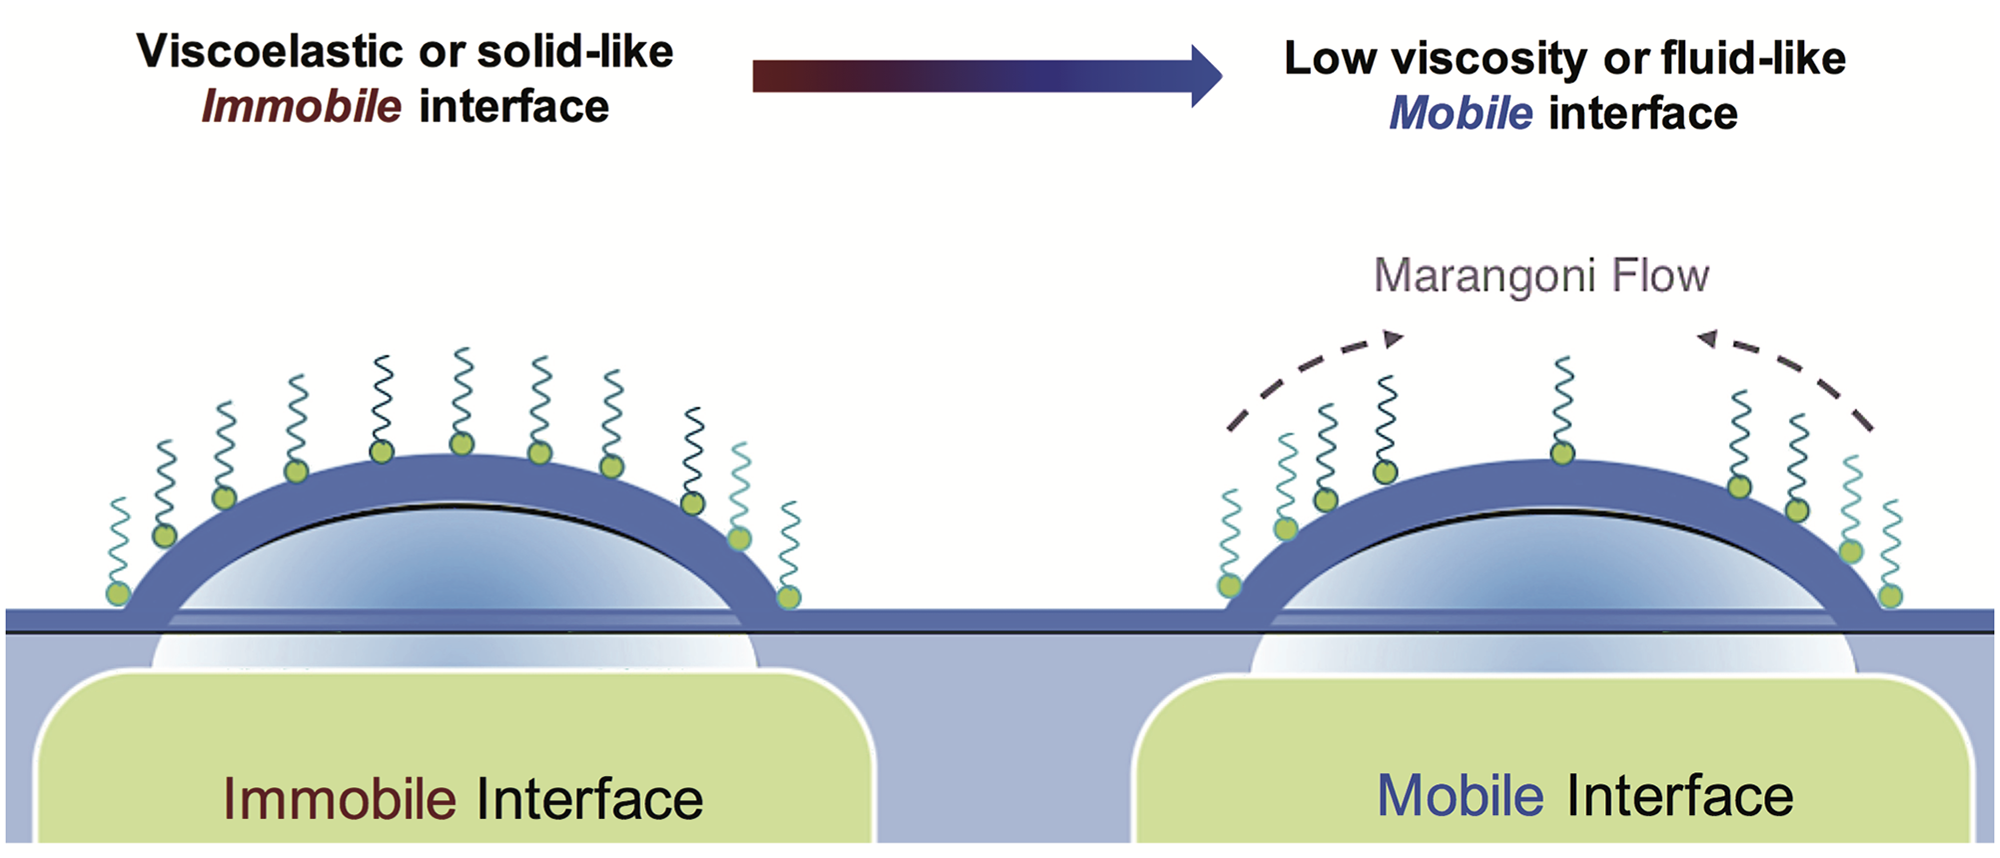
\includegraphics[scale = 0.8]{BhamlaFig8.PNG}
    \caption{Schematic shows the two surface regimes for surfactant laden thin films: "immobile" and "mobile" interfaces \cite{Bhamla2017}. The Marangoni flow induced by surface tension gradients depicted for mobile interfaces is further described in section \ref{sec:marangoni}.}
    \label{fig:Bhamla8}
\end{figure}

Surfactants with different solubility, surface viscosity and concentrations will tend to form two main classes of surfaces; "rigid" and "mobile" layers, as originally classified by Mysels in the 1960s \cite{Mysels1959Book}. For surfactants at lower concentrations (below the cmc), the adsorbed molecules are able to move easily along the surface, resulting in a "mobile" surface. These sometimes called "simple" mobile films \cite{Langevin1994} will exhibit complex turbulent motions, for instance seen in the colourful swirls appearing in common soap bubbles. On the other hand, at high concentrations, the molecules will form "rigid" and compact layers. These surfaces, deemed as "immobile" or static, will lead to slower drainage rates, and different stabilising effects \cite{Bhamla2017}. Structures formed by insoluble surfactants at high concentration, and soluble surfactants at high concentrations are slightly different, but exhibit similar phenomena \cite{Bhamla2017, ChampougnyNotBare2016}. At lower concentrations, insoluble surfactants will form visco-elastic surfaces whereas soluble surfactant laden surfaces can be assumed as inviscid \cite{Bhamla2017}. The two interfacial mechanisms can be seen represented in figure \ref{fig:Bhamla8}. Overall, the nature of surfactants used to stabilise a film has profound effects on the different drainage and rupture mechanisms it will experience, these include the possibility of marginal regeneration, and formation of a black film, which are discussed further in sections \ref{sec:marginalReg} and \ref{sec:blackfilms}.

\subsection{The Marangoni Effect}
\label{sec:marangoni}
Surface surfactant concentration and surface tension gradients are core characteristics which are extensively used in the study of thin films. It therefore comes as no surprise that the Marangoni effect would crop up in the explanations for a multitude of mechanisms described in this report. Indeed, this well studied phenomena discovered in the 1860s describes surface fluid mass flows driven by fluctuations in surface tension \cite{Marangoni1965}. Essentially, zones of decreased surface tension will tend to grow and move towards zones of increased surface tension.

Overall, this has the effect of stabilising thin films, as it tends to homogenise the distribution of adsorbed surfactant molecules. Indeed, a zone of higher surfactant concentration present on the film (due to temperature fluctuations, or other transient effects) will have a decreased surface tension value. This will induce a Marangoni flow which acts to spread the low surface tension zone, "compressing" and pushing higher surface tension zones away, spreading the surfactant molecules evenly \cite{Bhamla2017}. As seen in figure \ref{fig:Bhamla8}, this flow counters the bulk drainage flow direction, extending the bubble's lifetime. Naturally, the Marangoni effect is only observed for "mobile" film surfaces, as it requires the free movement of adsorbed surfactant molecules \cite{Langevin1994, Nierstrasz1999}.

\subsection{Discussion and Applications}
So far, this section has primarily focused on the main surface effects and structures observed in stable soap films. However, there are a multitude of other physical phenomena which could be looked into. Indeed, bubbles exhibit interesting behaviours when put into contact with EM fields, such as the Moses effect \cite{Wilson1925, Legchenkova2018}. Other significant effects include bubble coalescence events, where two bubbles first touch, and share a flat boundary, which thins and ruptures after a time, yielding a single, bigger bubble \cite{Pfeiffer2020}. These are particularly relevant to foams, and understandably play a large role in characterising their stability.

The thin nature of soap films allow them to be very useful when studying fluid flows. Indeed, they can often be approximated as two dimensional, making them the ideal testing ground for flow experiments. Two of these, reviewed by H. Kellay \cite{Kellay2017}, include testing models for friction drag using flowing thin films, and looking into turbulent effects such as vortices. The latter has significant applications as flows which appear on bubbles are comparable to atmospheric flows such as tropical cyclones \cite{Seychelles2008}.

\newpage
\section{Bubble Death and film rupture}
Thin films will experience a multitude of effects from the moment they are created, that weaken and push them to become unstable and eventually burst. In the following sections, these effects will be addressed chronologically: starting with initial drainage mechanisms which weaken the films, the moment rupture nucleates, to the dynamics and interesting fluid structures that develop around the newly formed accelerating hole, and finally what becomes of the fluid once the films have burst. As they exhibit many more interesting drainage and rupture mechanisms, this section will focus predominantly on surface bubbles in contact with their founding bulk fluid, while making sure to note when the effects are also relevant to "free" bubbles and films, and foams. The thin film part of the surface bubble is referenced as the "cap" and the edge at which it makes contact with the water is referenced as the "meniscus", "periphery" or "base" throughout.

\subsection{Film thinning mechanisms and rupture initialisation}
\label{sec:drainage}
All bubbles ranging from the ones formed with minimal surfactant concentrations (like tap water), which have lifetimes in the order of seconds \cite{Zheng1983, Lhuissier2011} to ones stabilised with high surfactant concentrations (well above the cmc) with lifetimes in the order of minutes or even hours, will exhibit film thickness reduction over time due to different drainage mechanisms. These effects cause fluid in the bubble's cap to be escape down into the bulk fluid on which the bubble is standing. These phenomena, dependant on the film's age, size and surfactant, will eventually lead the film thickness to reach some critical value and cause a hole to nucleate, sealing it's fate and beginning its annihilation.

\subsubsection{Gravity and capillary drainage}
\label{sec:GravNCap}
Gravity and capillary drainage are thinning mechanisms with occur regardless of the presence of surfactants adsorbed to the film and in the bulk solution. They typically appear for younger bubbles, right at the moment of their creation, before any stabilising surface tension gradients can be established \cite{Lhuissier2011}. The gravity driven drainage can simply be understood as the hydrostatic pressure generated by the mass of fluid in the bubble's cap, which will tend to push fluid out through the bubble's periphery and into the bulk fluid. Capillary drainage, driven by the capillary pressure inside the cap, acts more as a suction force which pulls liquid out of the cap. This effect occurs due to the thin nature of the film, and is caused by the surface tension of the fluid.

As pointed out by Lhuissier and Villermaux \cite{Lhuissier2011}, the relative importance of these two effects depends on the surface bubble's size. Smaller bubbles tend to be more spherical and sit lower into the bulk fluid, whereas larger bubbles will tend to the half-sphere shape, with their thin film cap being mostly above the bulk fluid level. Recalling the weight of fluid in the cap is very small, and often neglected in models \cite{Ida1998}, capillary pressure will therefore dominate for most bubbles bubbles which follow $R <= 5a$ \cite{Lhuissier2011}, where $a$ corresponds to the capillary constant and $R$ is bubble radius. This commonly used capillary length constant is a function of both gravity and surface tension. It can be noted here that this same capillary drainage mechanism also applies in foams \cite{Braun2002}, where instead of draining into the bulk liquid, fluid will drain from the films into what are called Plateau borders \cite{Almgren1976}. These are the edges at which the soap films, which constitute the foam, meet.

Regardless of whether hydrostatic or capillary forces are more significant, in both cases the drainage rates are relatively easy to compute, as they are simple pressure driven flows. A pressure gradient will drive liquid out of the cap, through the meniscus and into the bulk liquid (or directly into a Plateau border in the case of foams). In this regard, the Hagen-Poiseuille law or even very simple plug flow equations are used to determine the flowrate out of the cap, and therefore the thickness evolution of the film. Plug flow assumes a constant fluid velocity across the thickness of the cap, and was used by numerous authors, especially when negligible surfactant concentrations are considered \cite{Debregeas1998, Lhuissier2011, Breward2002, ChampougnyNotBare2016}. Poiseuille equations on the other hand take into account the velocity profile, with the effect of boundary conditions. They were used in the case where surfactants have formed a pair of rigid and immobile monolayers \cite{Nierstrasz1999, Bruinsma1995, Modini2013}, these are described in section \ref{sec:RigidMobile}.

The importance of surfactants in extending the lifetime of water surface bubbles specifically can now be clearly quantified. When no surfactants are present, the capillary and hydrostatic pressures lead to a very rapid drainage of water out of the cap. The only effect that can slow down this drainage is viscous stretching, where viscous forces oppose the thinning and deformation of the cap. However, this still leads to the drainage having characteristic times calculated using $\mu / \rho g L$, which yield values in the order of $10^{-4}$ s \cite{Breward2002, Lhuissier2011}. The "bare" water bubbles therefore appear to burst immediately. Noting how viscosity appears as a factor in the drainage time, G. Debregeas et al \cite{Debregeas1998} carried out drainage and bursting experiments on very viscous polymer melt and glass bubbles. This allowed them to study bubbles with significantly longer lifetimes (in the order of minutes), that admit essentially no surfactants as these are less easily adsorbed from the environment. Examining the cap thickness evolution for differently sized bubbles, they explained and effectively corroborated their results with plug flow equations utilising the capillary length. Extending these equations down to bare water bubbles, they also found similarly small characteristic times found by Breward and Lhuissier \cite{Breward2002, Lhuissier2011}. Overall this shows that for non-surfactant laden films, the thickness evolution can effectively be modeled by following the gravity and capillary drainage mechanisms.

\begin{figure}[!htbp]
    \centering
    \captionsetup{width=.9\linewidth}
    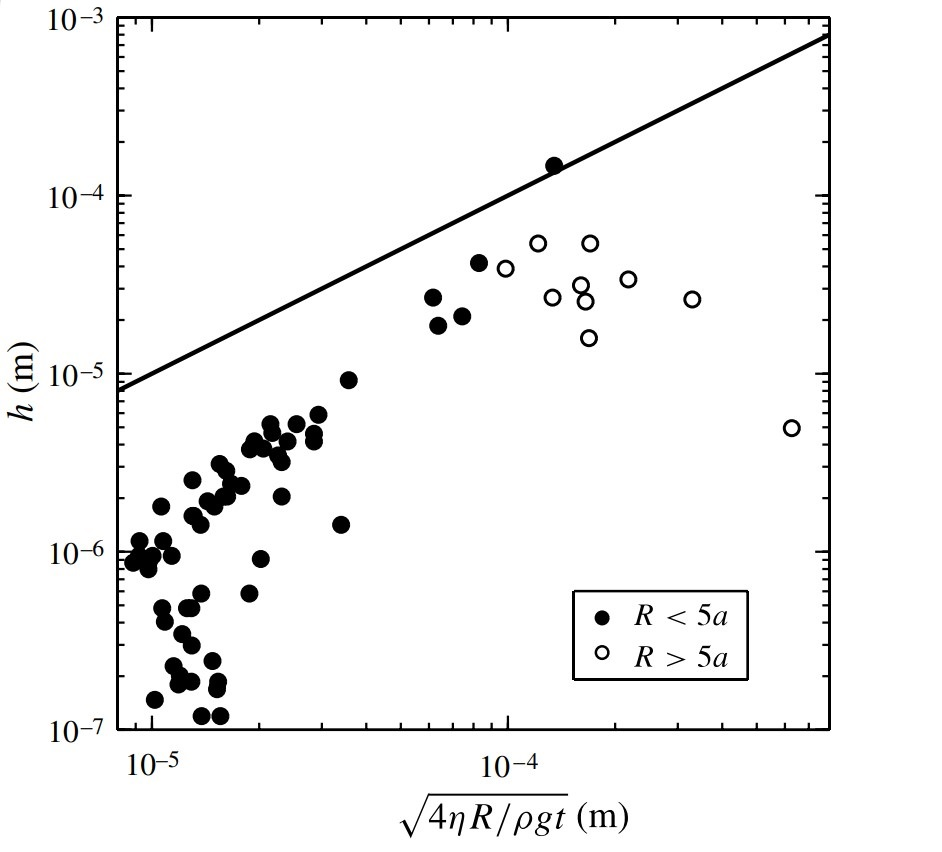
\includegraphics[scale = 0.5]{Fig_8_Lhuissier.jpg}
    \caption{Comparison of the drainage law which only includes Poiseuille flow, with experiments \cite{Lhuissier2011}. The law used clearly underestimates the actual physical drainage rates.}
    \label{fig:Lhuissier8}
\end{figure}

However, as seen in figure \ref{fig:Lhuissier8}, hydrostatic and capillary pressure driven drainage alone fail to model, and drastically underestimate, the thinning behaviour of films which do contain surfactants. Indeed, drainage seems to occur more rapidly than the expected Poiseuille flow. This discrepancy comes from an additional draining effect, marginal regeneration, which is studied in the next section (\ref{sec:marginalReg}).

\subsubsection{Marginal Regeneration}
\label{sec:marginalReg}

\begin{figure}[!htbp]
    \centering
    \captionsetup{width=.9\linewidth}
    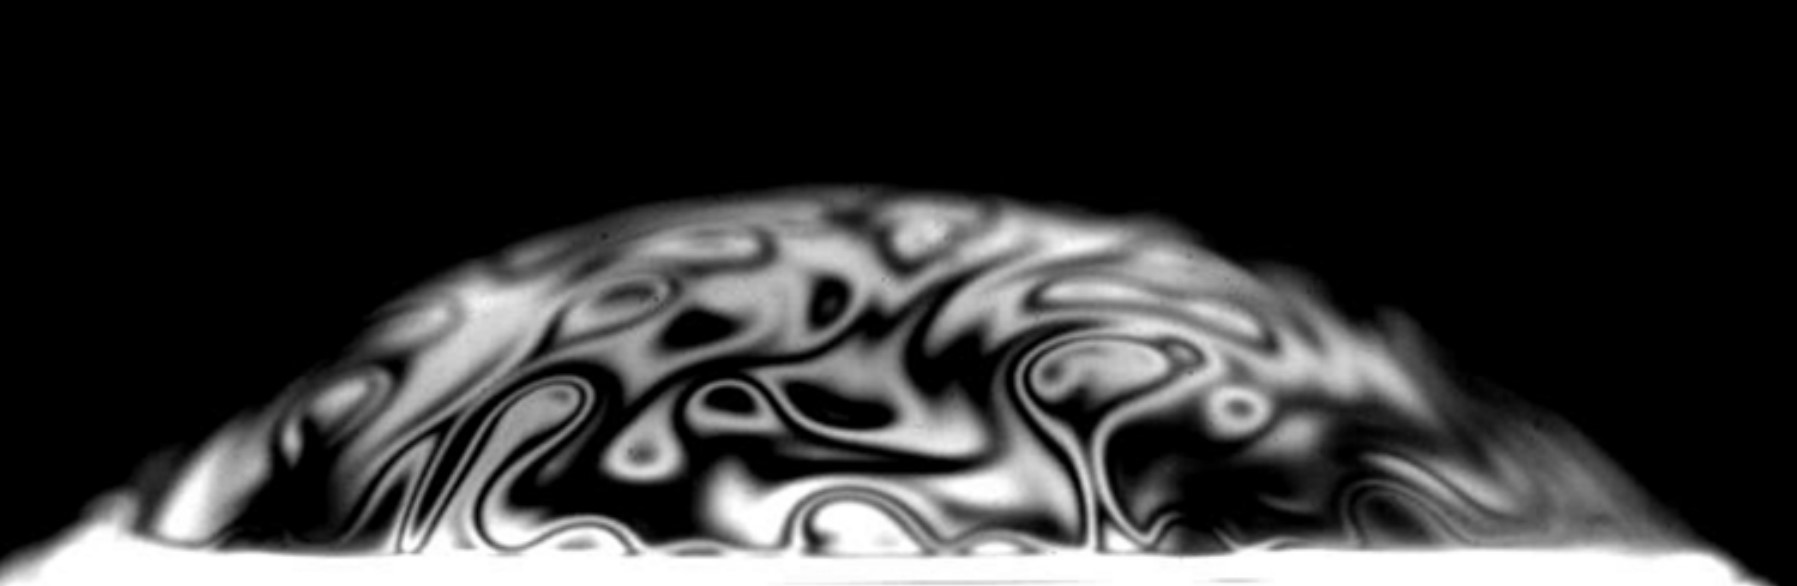
\includegraphics[scale = 0.4]{Fig_7_Lhuissier.jpg}
    \caption{View of a Bubble (radius R = 5 mm) under monochromatic lighting (sodium lamp at 589 nm) \cite{Lhuissier2011}. Fringes seen correspond to zones of constant thickness. Although they are usually studied in flat thin films, as it is easier to have a consistent light source pass through, here the convection plumes at the base of the film causing marginal regeneration can clearly be seen. }
    \label{fig:Lhuissier7}
\end{figure}

Marginal regeneration is a film drainage mechanism caused by the presence of free moving particles, like soluble surfactants, adsorbed at the surface of a thin film. First observed and introduced by Mysels in 1959 \cite{Mysels1959Book}, it results from the formation and movement of asymmetrical plumes of liquid along the base of films (and Plateau borders in foams \cite{Breward2002}), as seen in figure \ref{fig:Lhuissier7}. Observing the light interference fringes which appear when looking at a bubble from straight above, S. Bhamla et al were also able to clearly show these \cite{Bhamla2017}. Essentially, these additional fluid motions cause an additional liquid flux out of the bubble's cap, increasing its drainage rate. At relatively low surfactant concentrations, below the cmc, marginal regeneration is seen to dominate over the slower Poiseuille flows studied in section \ref{sec:GravNCap} \cite{Lhuissier2011, Bhamla2017}.

Physical explanations for these flows, and how they actually act to thin the bubble caps vary slightly for different authors \cite{Nierstrasz1999, Bhamla2017, Lhuissier2011, ChampougnyNotBare2016, Bruinsma1995}. Originally, Mysels \cite{Mysels1959Book} believed these were caused by small thickness variations caused by thermal effects. However, more recent studies all agree on one point: the complex flows observed are driven by surface tension gradients. S. Bhamla et al \cite{Bhamla2017} explain the surface flow by arguing that as a plume is created along the surface of the film, its head causes the film to dilate and "creates a new surface area", which decreases the surface concentration of surfactants, hence creating a zone of higher surface tension. This will result in more liquid being pulled from the bulk towards the depleted zone, essentially further fueling the motion. Although this explanation doesn't outwardly specify it, it is important to note that these plumes are zones of decreased thickness, which act to drain the film as thicker zones are drawn into the bulk fluid \cite{Lhuissier2011, Nierstrasz1999}, as seen in figure \ref{fig:BruinsmaMerge}. R. Bruinsma et al \cite{Bruinsma1995} attribute the movement to buoyancy forces. They also underline that the flow from the film to the meniscus not only deposits fluid, but also surfactant molecules. Furthermore, fluid pulled from the bulk liquid up into the film has a lower surfactant concentration, because as mentioned before surfactants are drawn to fluid boundaries. The surface concentration of surfactant molecules is generally higher than the concentration in the bulk fluid \cite{Gast1997}.

\begin{figure}[!htbp]
    \centering
    \captionsetup{width=.9\linewidth}
    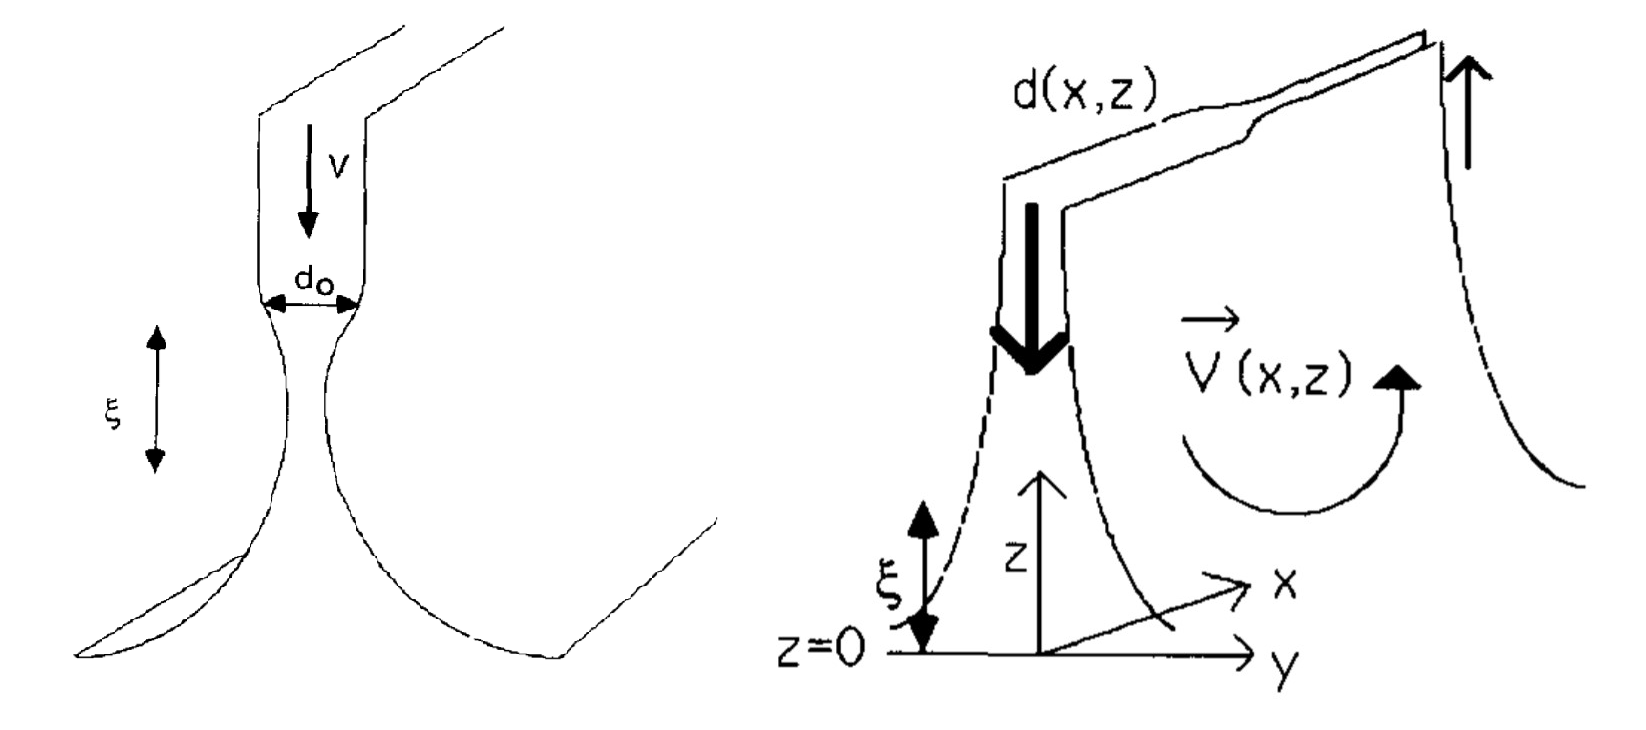
\includegraphics[scale = 0.35]{BruinsmaFigMerged.jpg}
    \caption{On the left: Diagram of the thinned zone caused by marginal pinching, with characteristic lengths used to setup the drainage laws. On the right: Marginal regeneration flows at the bottom of a film, thicker regions move down into the meniscus while thinner region (plumes) rise up into the film. \cite{Bruinsma1995}}
    \label{fig:BruinsmaMerge}
\end{figure}

The actual inception of these plumes, or "patches" as characterised by Champougny et al \cite{ChampougnyEvap2018}, can be attributed to the existence of a pinching region, seen in figure \ref{fig:BruinsmaMerge}. This thin zone quickly appears along the base of the bubble cap by a process called 'marginal pinching' \cite{Joye1994, Aradian2001}, and its destabilisation causes the plumes to be formed. Simply put, the pressure inside of the meniscus (or Plateau border) is lower than the capillary pressure exerted by the thin film. This difference is what generates the flow out of the cap, but it also causes marginal pinching. According to Lhuissier and Villermaux \cite{Lhuissier2011}, the relatively large surface tension gradient difference between the two sides of the thinned zone is what causes the Benard-Marangoni destabilisation triggering marginal regeneration.

Overall, models which take the marginal regeneration effect into account can be established, either by coupling it directly with capillary pressure \cite{Lhuissier2011}, by considering mass balances for both surface, intralamellar (between the two surfactant monolayers) and bulk fluid \cite{Nierstrasz1999}, or by applying boundary conditions and assumptions to existing surface models (like the Boussinesq-Scriven model) \cite{Bhamla2017}. These generally yield solutions which are much closer to experimental values.

\subsubsection{Newton Black films}
\label{sec:blackfilms}

You might have encountered this curious state when observing floating soap bubbles. In the seconds before their death, they sometimes becomes practically invisible, no longer exhibiting colourful interference patterns. In certain cases before rupture, as the drainage mechanisms cause liquid to leave the film, there will be a limit at which thickness becomes very small (5 to 10nm), and the film stabilises. This resulting extremely thin metastable equilibrium is referenced as Newton (NBF) or common "Black" film (CBF), as A. Vrij and J. Th. G. Overbeek explain: "black, because interference between light reflected from the front side and that reflected from the back side leads to nearly complete extinction of the reflected light" \cite{Vrij1968}. The films aren't actually black per se, they just happen to reflect such little light that they appear invisible \cite{Langevin1994}, or black in front of a black backround. Here, this equilibrium state is qualified as metastable as it is very sensitive to external fluctuations. These films are found to appear in higher surfactant concentration bubbles, above the cmc \cite{Bhamla2017, Manev1974}, in patches located towards the apex of bubbles before rupture. This is understandable, as the film is usually thinnest at those locations. In a recent research article attempting to develop a model for describing these patterns observed at the surface of surfactant-laden bubbles, L. Shen et al \cite{Shen2020} describe these regions as "black holes". They characterise these to be in a close packing configuration, where the maximum amount of surfactant molecules have adsorbed to the surface. This can be recognised as the critical micelle concentration described earlier, and agrees with the previous works which noticed the formation of black films at similarly high concentrations \cite{Bhamla2017, Manev1974}.

This unexpected stability is often said to come from a balance of the capillary suction with intermolecular interactions (they become non-negligible at this thickness) \cite{Breward2002, ChampougnyEvap2018, Cantat2010, Vrij1968, VrijDiscussion1966}. The intermolecular forces at work are: the electrostatic repulsion and van der Waals attractions of the molecules from the two boundaries of the surfactant bilayer, and the "hard-core" repulsion of the molecules themselves when the film is at its thinnest \cite{Casteletto2003}. Note that the overall sign of the intermolecular interactions should be repulsive for black films to form. If they are not, they will accelerate the thinning and cause rupture, desabilising the film instead of stabilising it \cite{VrijDiscussion1966, Langevin1994, Debregeas1998}. It should be restated here that black films can be categorised in two forms: the thicker "common" black film (10 nm), and the thinnest possible "Newton" black film, which has a typical thickness of only two surfactant molecules (roughly 4-5 nm) \cite{Casteletto2003, Seung2006}. Interestingly, V. Casteletto et al \cite{Casteletto2003} noticed and studied and apparent hysteresis in the CBF-NBF transition. Indeed, by varying the internal pressure of a soap film created on the end of a small hole (2 mm), and measuring its thickness via interferometry, they were able to find a range of pressures at which either of CBF and NBF could be observed. This previously undocumented non-linear nucleation effect could be linked back to the spontaneous thickness changes which were observed and analysed by A. Vrij and J. Th. G. Overbeek 50 years prior \cite{Vrij1968}.

Most experiments described in this report neglect, or do not take into account the effect of ambient humidity and evaporation in their models \cite{Manev1974, Zheng1983}. Only a few mention in passing its "importance" or controlling it, but without citing its effects \cite{Langevin1994}. Intuitively, it could be perceived that at such small thicknesses, this external flux could potentially have an impact. In a recent 2018 paper, L. Champougny et al \cite{ChampougnyEvap2018} studied this effect by measuring the maximum length reached by a flat film pulled at constant velocity until rupture, for different ambient humidity. Surprisingly, they found a positive correlation between humidity and critical film length. However by closer observing the thinning dynamics, they did not find evaporation to affect these, this lead them to believe evaporation only starts to become significant very close to rupture.


\subsubsection{Rupture initialisation}
Now that we have examined the thinning effect of drainage mechanisms, the following questions arise: what triggers the film to actually begin rupturing, why don't all films thin down to black film thickness, and why can't they remain so indefinitely? Overall, the theories outlined below all attempt to find a value for the "critical thickness" of the film at the onset of bursting. This somewhat simple value, when linked with the thickness evolution equations derived from the drainage mechanisms, could be used to predict the film's lifetime.

Black films are believed to rupture unpredictably due to the lack of control over the environment: thermal shocks, vibrations, dust, or as recently observed, evaporation \cite{ChampougnyEvap2018}. Recently, Lhuissier and Villermaux \cite{Lhuissier2011} considered a statistical approach by admitting a frequency of thermal fluctuation events from the environment, where an activation energy would cause rupture (this is the nucleation energy for the creation of a hole at the surface). Although this was able to successfully estimate the lifetime for black films, it yielded non-physical values for thicker films. For these non-black films, the energy of activation for nucleating a hole is considered too large for these phenomena to have an effect \cite{VrijDiscussion1966}. Instead, thermal fluctuations in the environment were believed to cause surface "corrugations" (variations in thickness) to appear \cite{Vrij1968, VrijDiscussion1966}, which grow over time, and when a critical wavelength is reached, to cause spontaneous rupture. Vrij developed a popular model for this wavelength, based on surface tension and the "Free energy of interaction", being the long-range intermolecular forces acting in the surfactant bilayer. Although this model was able to somewhat accurately predict critical thicknesses for certain experiments at the time, it incorrectly models the effect of bubble radius and surface tension for more recent experiments \cite{Langevin1994}. As Vrij admits, his model did not include the complex movement of surfactant molecules at the surface, and their role in surface elasticity. The latter was later proven to be an important factor in describing critical thickness by D. Langevin and A.A. Sonin in 1994 \cite{Langevin1994}.

More recent advancements made in understanding the marginal regeneration effect for example \cite{Bhamla2017}, have led alternative explanations to be explored as a substitute for thermal effects. These include its role in catalysing turbulent flows along the surface of bubbles which, following an energy scale analysis, could show rupture is a possible consequence (albeit unconvincingly \cite{Lhuissier2011}). Alternatively, Lhuissier and Villermaux also observed that nucleation of holes in tap water bubbles occurred predominantly at "convection cells" \cite{Lhuissier2011}, these are the rising plumes described in section \ref{sec:marginalReg}. This seems rather evident, as these are known to be zones of reduced thickness. They developed a model which revolves around probabilities for a thin enough plume to rupture, which turned out to be a function of the capillary length scale. Although this model does fit well with experiments \cite{Modini2013}, it still relies on a probability factor they call the "puncture efficiency". This value has no current physical relationship and is experimentally derived. This makes their solution appear more like probability fitting rather than being rooted in physically explained mechanisms. In parallel, more recent studies have considered models based on molecular dynamics simulations \cite{Nguyen2014}, or further investigations into the thermal effects \cite{Shah2019}. However, although experiments over the years have provided a thorough quantitative understanding of the phenomena, none have been able to provide a solely qualitative model to explain the critical thickness and onset of rupture in thin films.

\begin{figure}[!htbp]
    \centering
    \captionsetup{width=.9\linewidth}
    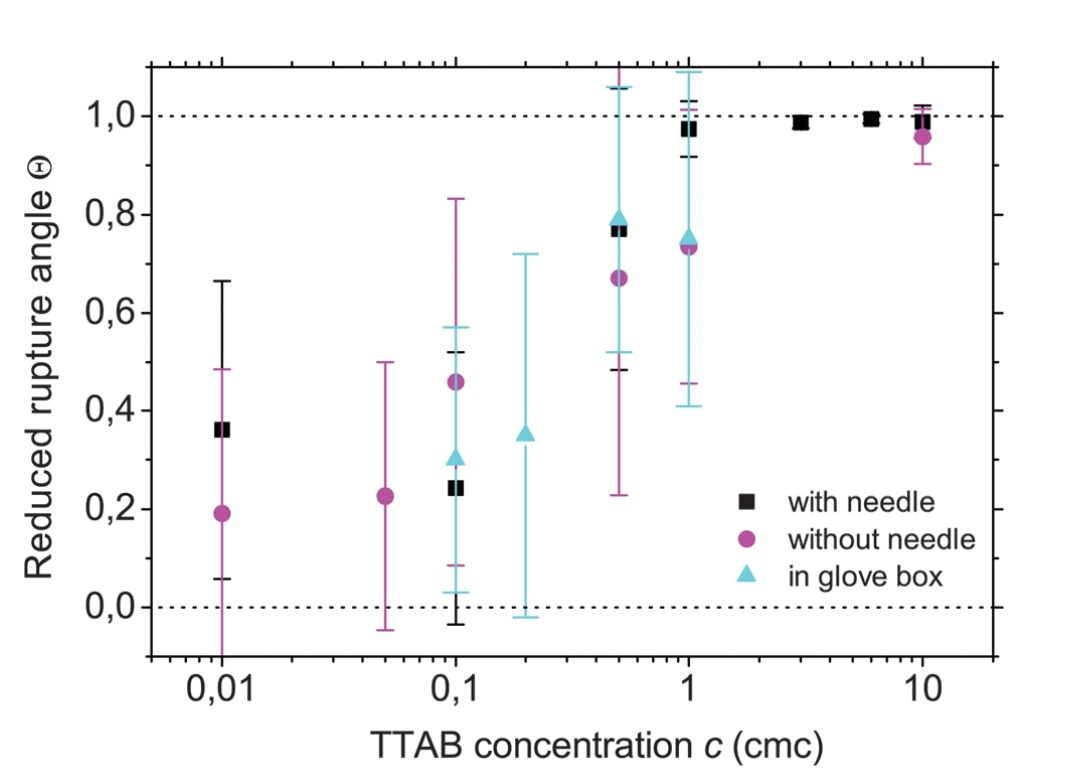
\includegraphics[scale = 0.5]{ChampougnyFig10.jpg}
    \caption{Reduced rupture angle $\Theta$ (0 corresponds to a rupture nucleated at the meniscus, tends to 1 as the point approaches the apex of the bubble) as a function of TTAB surfactant concentration, normalized with respect with its cmc. Each symbol corresponds to a different experimental condition, and each point shows the average and standard deviation for 4 to 20 bubbles. Figure adapted from \cite{ChampougnyNotBare2016}.}
    \label{fig:ChampougnyFig10}
\end{figure}

Despite this, an interesting remark can be made for the position of the nucleated hole along the bubble surface. Overall, it seems that when marginal regeneration is the driving drainage mechanism, bubbles will tend to burst from a point close to their periphery \cite{Bhamla2017, Lhuissier2011}. On the other hand, "bare" bubbles, and bubbles with immobile surfactant surfaces (section \ref{sec:RigidMobile}) tend to burst at their apex. Champougny et al \cite{ChampougnyNotBare2016} carried out experiments to study this effect, which yielded figure \ref{fig:ChampougnyFig10}. This data clearly shows with relative certainty that high surfactant concentration bubbles do indeed burst at their apex. This can be explained by the monolayers becoming "saturated", resulting in immobile surfaces which only exhibit the symmetric gravity and capillary drainage mechanisms \cite{Bhamla2017}. This symmetry implies the hole can only appear at the apex. Values for lower concentrations however come with large uncertainties, and are reminiscent of the stochastic nucleation behaviour caused by marginal regeneration. In this aspect, a probabilistic model is required to predict the position of the nucleation hole. In short, the rupture behaviours for mobile surfactant films have yet to be fully defined, and it is difficult to do so due to the stochastic nature of the problem.

\subsection{Hole Development}

\begin{figure}[!htbp]
    \centering
    \captionsetup{width=.9\linewidth}
    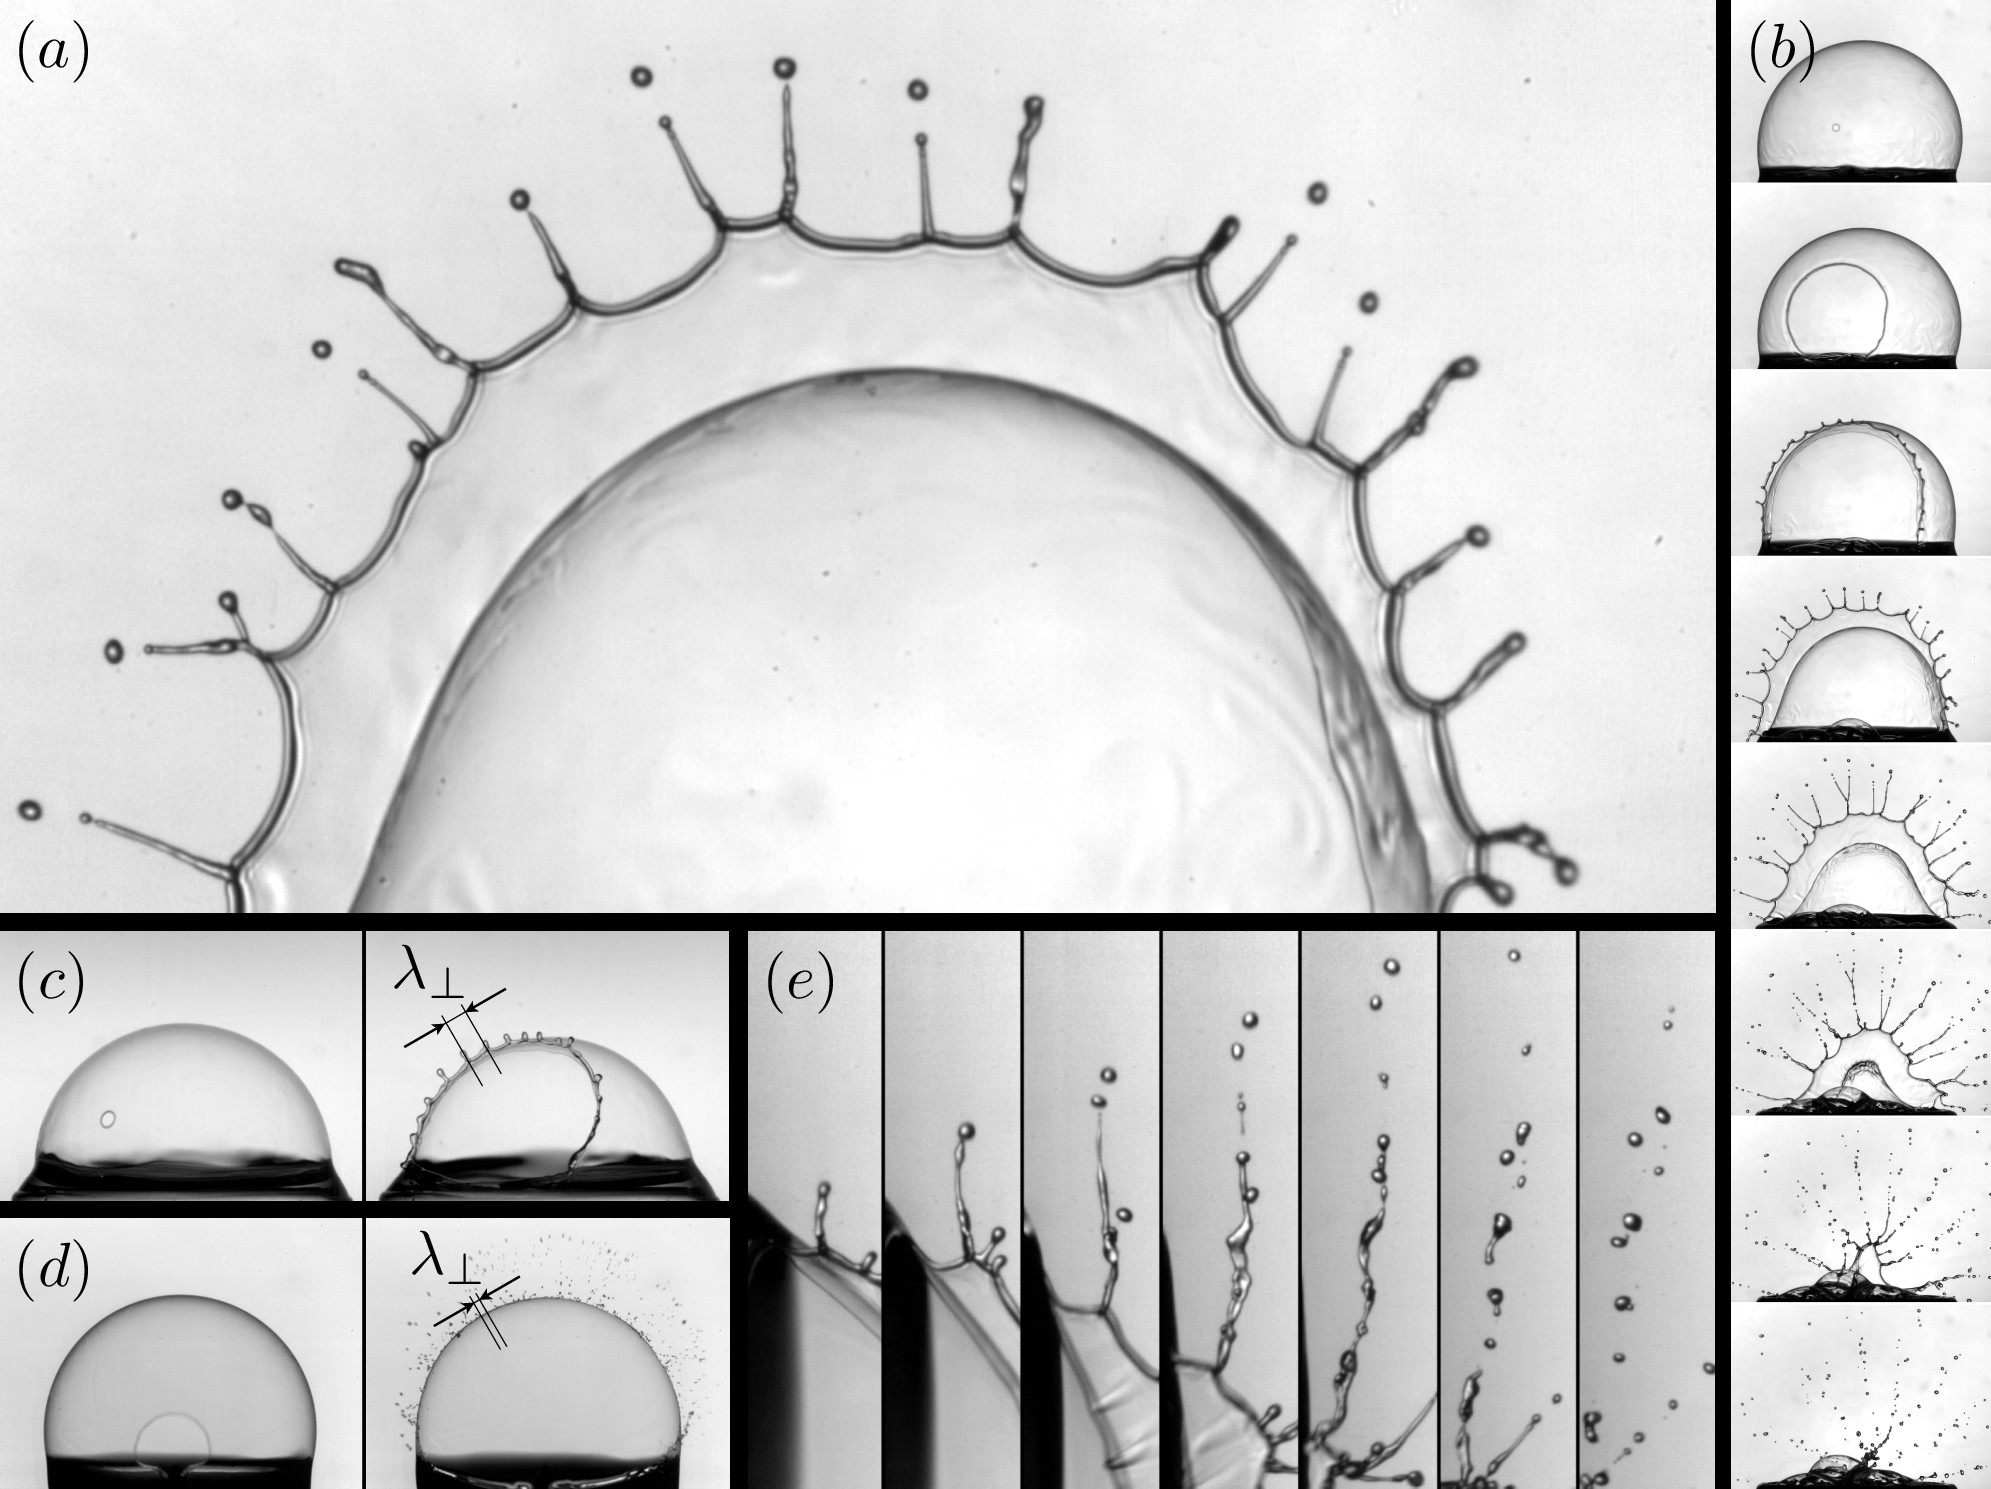
\includegraphics[scale = 0.21]{Lhuissier2009.jpeg}
    \caption{Fluid structures emerging from the opening rim of the nucleated hole in a soap bubble \cite{Lhuissier2009}.}
    \label{fig:Lhuissier2009}
\end{figure}

Now that a hole has nucleated somewhere along the bubble's surface, it will start to grow and widen, accumulating fluid in its rim until instabilities grow and cause it to fragment into a multitude of fluid structures and droplets. These steps can be admired in figure \ref{fig:Lhuissier2009}. Although this behaviour might not seem to be directly linked to stability (as the bubble is already doomed), the dynamics of film rupture are very interesting and have significant impacts for their applications. Indeed, bubbles play a key role in the production of natural and man-made aerosols \cite{Lhuissier2011, Modini2013}. On top of this, if the dynamics of hole opening can be well defined, this could give more insight into the process causing its nucleation.

\subsubsection{Rim Velocity}

\begin{equation}
    \label{eq:TaylorCulick}
    v = \sqrt{\frac{2 \sigma}{h \rho}}
\end{equation}

The rim velocity pertains to the velocity of the initially circular opening hole now present in the film. Primitively derived by Rayleigh using a simple energy balance \cite{Rayleigh1902}, it was first improved by Taylor and Culick independently to include the inertia of the liquid accumulating at the "rolling edge" \cite{Taylor1959, Culick1960}. This known as the Taylor-Culick velocity, available in equation \ref{eq:TaylorCulick}, where $\sigma$ is surface tension, $h$ is the film thickness at rupture (assumed uniform), and $\rho$ is the liquid density. Although, as we will see, this model is known to overestimate rim velocities over time, it is a good approximation for the immediate velocity of the opening hole for relatively low viscosity fluids, like water \cite{Brenner1999, Lhuissier2011}. Recent papers still often utilize this model, for example to verify the critical film thickness \cite{Modini2013, Debregeas1998}. The opening velocity can also be used to estimate the surface elasticity \cite{Petit2015}.

\begin{figure}[!htbp]
    \centering
    \captionsetup{width=.9\linewidth}
    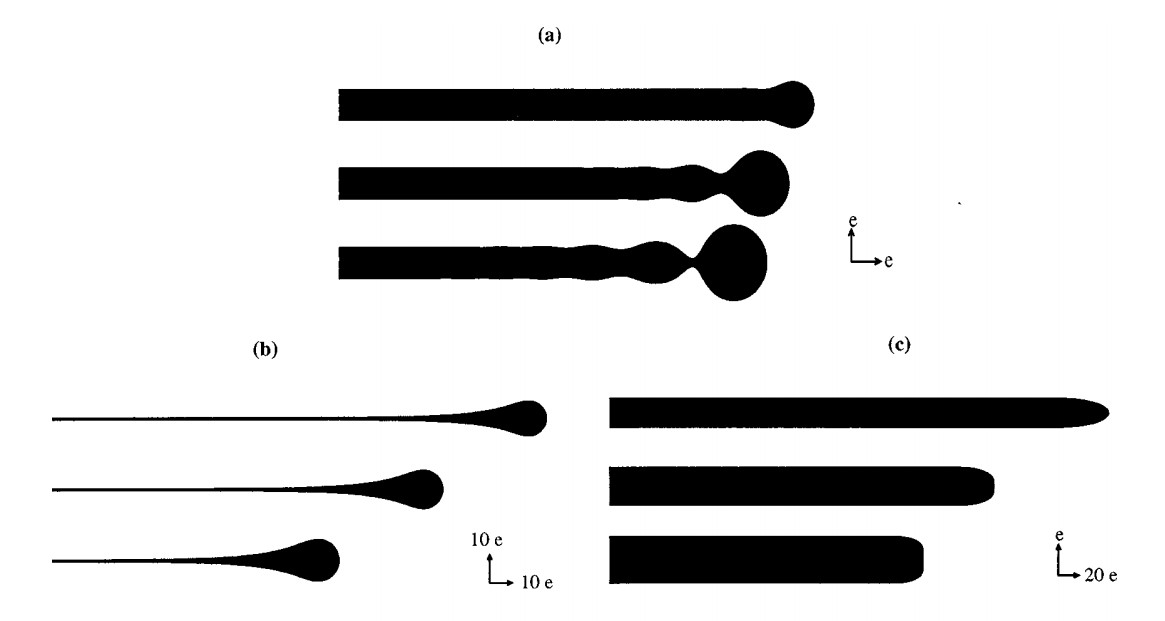
\includegraphics[scale = 0.6]{BrennerFig1.jpg}
    \caption{Film retraction profiles for (a) $Oh ~ 10^{-6}$ (b) $Oh~ 10^{2}$ (c) $Oh~ 10^{8}$. Arrow lengths are given in terms of film thickness $e$. Here, the absence of fluid accumulation for high $Oh$, and appearance of capillary wave disturbances ahead of the edge for low $Oh$ can clearly be seen \cite{Brenner1999}.}
    \label{fig:Brenner1}
\end{figure}

A known fact about the Taylor-Culick velocity is that it neglects the viscosity. Since the Reynolds number for the flow is generally very high, the effect of surfactants and molecular scales are expected to be negligible \cite{Petit2015, Brenner1999}. However, for high viscosity fluid films, or "sheets", this is not the case, and slower retraction behaviours deviate from the usual. First looked into by Debregeas and de Gennes in 1998 \cite{Debregeas1998}, these have been studied extensively since \cite{Brenner1999, Savva2009}. Interestingly, for bare high viscosity films, fluid doesn't accumulate in the rim and the radius of the hole actually grows exponentially. \cite{Debregeas1998}. Debregeas et al \cite{Debregeas1998} explain this behaviour by arguing that since opening velocities are small, surface tension forces are able to propagate through the film and smooth out the rim. In effect, they argued that the absence of fluid buildup at the rim was due to the viscoelastic properties of the film. A following work by M. Brennder and D. Gueyffier \cite{Brenner1999} showed that the absence of a rim could also be explained through a viscous effect alone. Both explanations seem to hold up equally, and yield similarly accurate models.

Here, it is useful to introduce a non-dimensional number which appears commonly in thin film problems: the Ohnesorge number $Oh$, which expresses the relative effects of viscosity and surface tension. This number allows us to determine which retraction regime a bubble might have: at low $Oh<0.1$, "capillary wave disturbances" can be observed ahead of the rim which accumulates liquid , whereas at high $Oh>10$, viscosity dominates, and no rim is formed \cite{Savva2009, Brenner1999}. These effects are shown schematically in figure \ref{fig:Brenner1}.

Going back to lower viscosity films, explanations for the slight deviations from the Taylor-Culick velocity vary. In a 2015 paper, P. C. Petit et al \cite{Petit2015} observed large deviations from the usual Taylor-Culick rim velocity and crack-like patterns for films with high surface rigidity. This rigidity meant surfactant particles did not have time to diffuse from the surface into the film as it was being compressed. Petit et al called this a "compressive shock", which caused cracks or folds to appear away from the rim. These new fluid structures and discontinuities led to an additional energy loss, resulting in slower rim velocities than expected. A popular cause for the deviation from the Taylor-Culick velocity is often attributed the formation of other disturbances ahead of the rim, known as the "aureole" \cite{McEntee1969, Bico2015, Muller2009}. These are believed to be caused by an accumulation of surfactant particles in the travelling rim, which leads to the formation a surface tension gradient. Since the rim has accumulated a higher concentration of surfactant molecules, it has a lower surface tension with respect to the yet undisturbed film. This is characterised by the disturbance (aureole). For the case of bubbles, some proposed that the apparent decrease in velocity is caused by the rim moving towards regions of increased thicknesses \cite{Mukerjee1971, Debregeas1998}. If the hole nucleates at the apex of the bubble, this does seem like a very sensible reasoning. Other less frequent explanations point to small fluid particles ejected from the rim \cite{Muller2009} or the elongated circular shape of the rim \cite{Bico2015}.

\subsubsection{Appearance of instabilities}
For low viscosity soap bubbles, viscous and surface tension forces are too weak to sustain the rim's circular shape over time as it accelerates and accumulates fluid. This causes it to exhibit an inertial destabilisation \cite{Lhuissier2011}, leading to the formation of ligaments and ejecting fluid particles. These structures are clearly seen in figure \ref{fig:Lhuissier2009}. Observing the evolution of the ligaments in that figure, they can be seen to break up into single droplets. This can be described by a Plateau-Rayleigh instability \cite{Lhuissier2011}, the same instability which can be observed in flow coming out of a tap: at some distance away from the tap's outlet the stream always breaks up into droplets. This results from the action of surface tension to minimise surface area \cite{Rayleigh1878}. At high viscosity however, due to the relatively slower bursting dynamics, a different instability can be observed. Indeed, Debregeas et al \cite{Debregeas1998} describe the formation of a "parachute instability", where the bubble would deflate and crumple under its own weight before the rim could reach the bubble's base. This results in ridges being formed along the surface, where similarly to the cracks and folds observed in rigid films by Petit et al \cite{Petit2015}, the film appears to behave like an elastic sheet.

\subsection{The aftermath}

\subsection{Applications}

\subsection{Discussion}

Marginal regeneration was only specifically observed in surface bubble and foams, and examples of it occurring in free floating spherical bubbles couldn't be found. However, knowing that fluid generally builds up at the base of concave films \cite{Shen2020}, we could expect a similar drainage flow to appear at that point. Instead of forming a convecting flow with its bulk fluid, or a plateau border, it could form this mass flux with this built-up fluid mass.

Overall, drainage mechanisms and film rupture are a priori linked, as thinner films are more likely to rupture. Nevertheless, the onset of bursting, although quantitatively well described is not yet fully understood. Further research is required to truly understand the physical phenomena causing thicker films to rupture (thicker than black films), and develop satisfactory models which can be applied generally.


%\newpage
\section{Improving stability}
Overall, we have seen that a bubble will exhibit stabilising phenomena such as the Marangoni effect, as well as a multitude of mechanisms which act to weaken their thin films. These include plug-flow-like capillary and hydrostatic pressure driven drainage, often quicker draining marginal regeneration effects, and ultimately the nucleation of a hole at its surface. Along the way, some controllable parameters which can be used to increase a bubble's stability have been identified. These are discussed below, considering bubble lifetime as a metric for bubble stability.

The addition of surfactants to a pure or "bare" thin film will always increase its stability. The introduced molecules will adsorb to the interfaces, forming supporting and protective monolayer and bilayer structures \cite{Gast1997, Mysels1968Nomenclature}. In an attempt to maximise bubble lifetime, the use of an insoluble surfactant at high concentrations will generally yield more stable bubbles \cite{Petit2015, ChampougnyNotBare2016, Bhamla2017}. Indeed, these form rigid surfaces which drain significantly slower. Due to their high surface viscoelasticiy, the surfactant molecules are slow to move across the film's surface, marginal regeneration does not occur, and the driving drainage mechanism is reduced to the much slower Poiseuille flow. Regardless of the solubility of the surfactant using it at high concentrations, up to their critical micelle concentration (cmc), will further "stiffen" the film surfaces \cite{Bhamla2017}. A "stiffer" film interface will tend to be more stable as its drainage dynamics are slower. This added stiffness is can be characterised as the surface pressure (difference between surfactant-laden and "bare" file surface tensions).

When using the more common soluble surfactants, diffusivity becomes relevant for bubble stability \cite{deGennesYoung2001}. This factor dictates the speed at which molecules can diffuse to an interface. This is relevant as when exposed to external fluctuations like stretching, it is important that the surfactant molecules in the fluid between the surfaces adsorb to the newly created surface. In essence, this coefficient affects how easily the film can recover to external perturbations.

If for a certain reason, surfactants are not an option, then higher viscosity fluids should be used. These create "bare" films which approximately drain following a capillary characteristic time, a function of viscosity. For example, if a fluid with more than a million times the viscosity of water is used to make a bubble, it can have lifetimes in the order of minutes \cite{Debregeas1998}. This is opposed to the fact that pure water bubbles die practically instantly (approx. $10^{-5} s$) \cite{Lhuissier2011}. On top of this, following a recent study, ambient evaporation could have an effect on the dynamics of rupturing films at rupture \cite{ChampougnyEvap2018}. This implies that the bubbles' environment should be humid, or relatively cold, in order to reduce the additional flux caused by evaporation. However, further research is required as the results aren't conclusive, and this effect seems to only be relevant at and close to rupture.

Theoretically, if all temperature fluctuations, dust and other external disturbances could be controlled, there is one film that could remain stable indefinitely: the Black film studied in section \ref{sec:blackfilms}. Indeed, with thicknesses down to a few surfactant molecules \cite{Casteletto2003}, these films reach a metastable equilibrium between repulsive intermolecular interactions and capillary pressures \cite{Breward2002, ChampougnyEvap2018, Cantat2010, Vrij1968, VrijDiscussion1966}. However, such controlled environments are non-existent, meaning these types of films seem unlikely to be viable.

%\newpage
\section{Conclusions}
In conclusion, thin fluid films in the form of surface bubbles exhibit a range of effects in their lifetime. These are often comparable to free bubbles, foams and flat films. They are stabilised by adsorbed surfactant amphiphiles, which affect interfacial rheology and surface tension, forming monolayers which admit a certain mobility. Over time, film thickness reduces down to a critical value, due to fluid draining out of the bubble's cap. When the film surfaces are mobile, this thickness evolution can be derived from marginal regeneration drainage laws. On the other hand, immobile surfaces drain slowly, following Poiseuille flows.



\newpage
\singlespacing
%\small% <- use this to make smaller text if space needed
\bibliographystyle{IEEEtran}
\bibliography{papers}

%The Bee movie. (2007). [film] Directed by J. Seinfeld. DreamWorks Animation.

\includepdf[noautoscale=true, width=\paperwidth]{2020-21 ME3-hLTR Meeting Log_Pierre.pdf}
\end{document}
